\section{Interrupciones}

Con el uso de interrupciones, el procesador puede dedicarse a ejecutar otras instrucciones mientras una operación de E/S está en curso. El procesador puede ser notificado cuando la operación de E/S ha terminado, y puede continuar con la ejecución de la instrucción que se interrumpió.
Cuando el dispositivo externo está listo para aceptar maás datos del procesador, el módulo de E/S de este dispositivo externo envía una señal de \textit{petición de interrupción} al procesador. El procesador responde suspendiendo la operación del programa que estaba ejecutando y salta a un programa, conocido como gestor de interrupción, que da servicio a ese dispositivo concreto, y prosigue con la ejecución del programa original después de haber dado dicho servicio al dispositivo.

Para permitir el uso de interrupciones, se añade un \textit{ciclo de interrupción} al ciclo de instrucción. En el ciclo de interrupción el procesador comprueba si se ha generado alguna interrupción, indicada por la presencia una señal de interrupción. Si no hay señales, el procesador contonúa con el ciclo de captación y accede a la siguiente instrucción del programa. Si hay alguna petición, el procesador suspende la ejecución del programa en curso y guarda su contexto. El procesador carga el contador de programa con la dirección de comiento de una rutina de interrupción.

\begin{figure}[h]
  \centering
  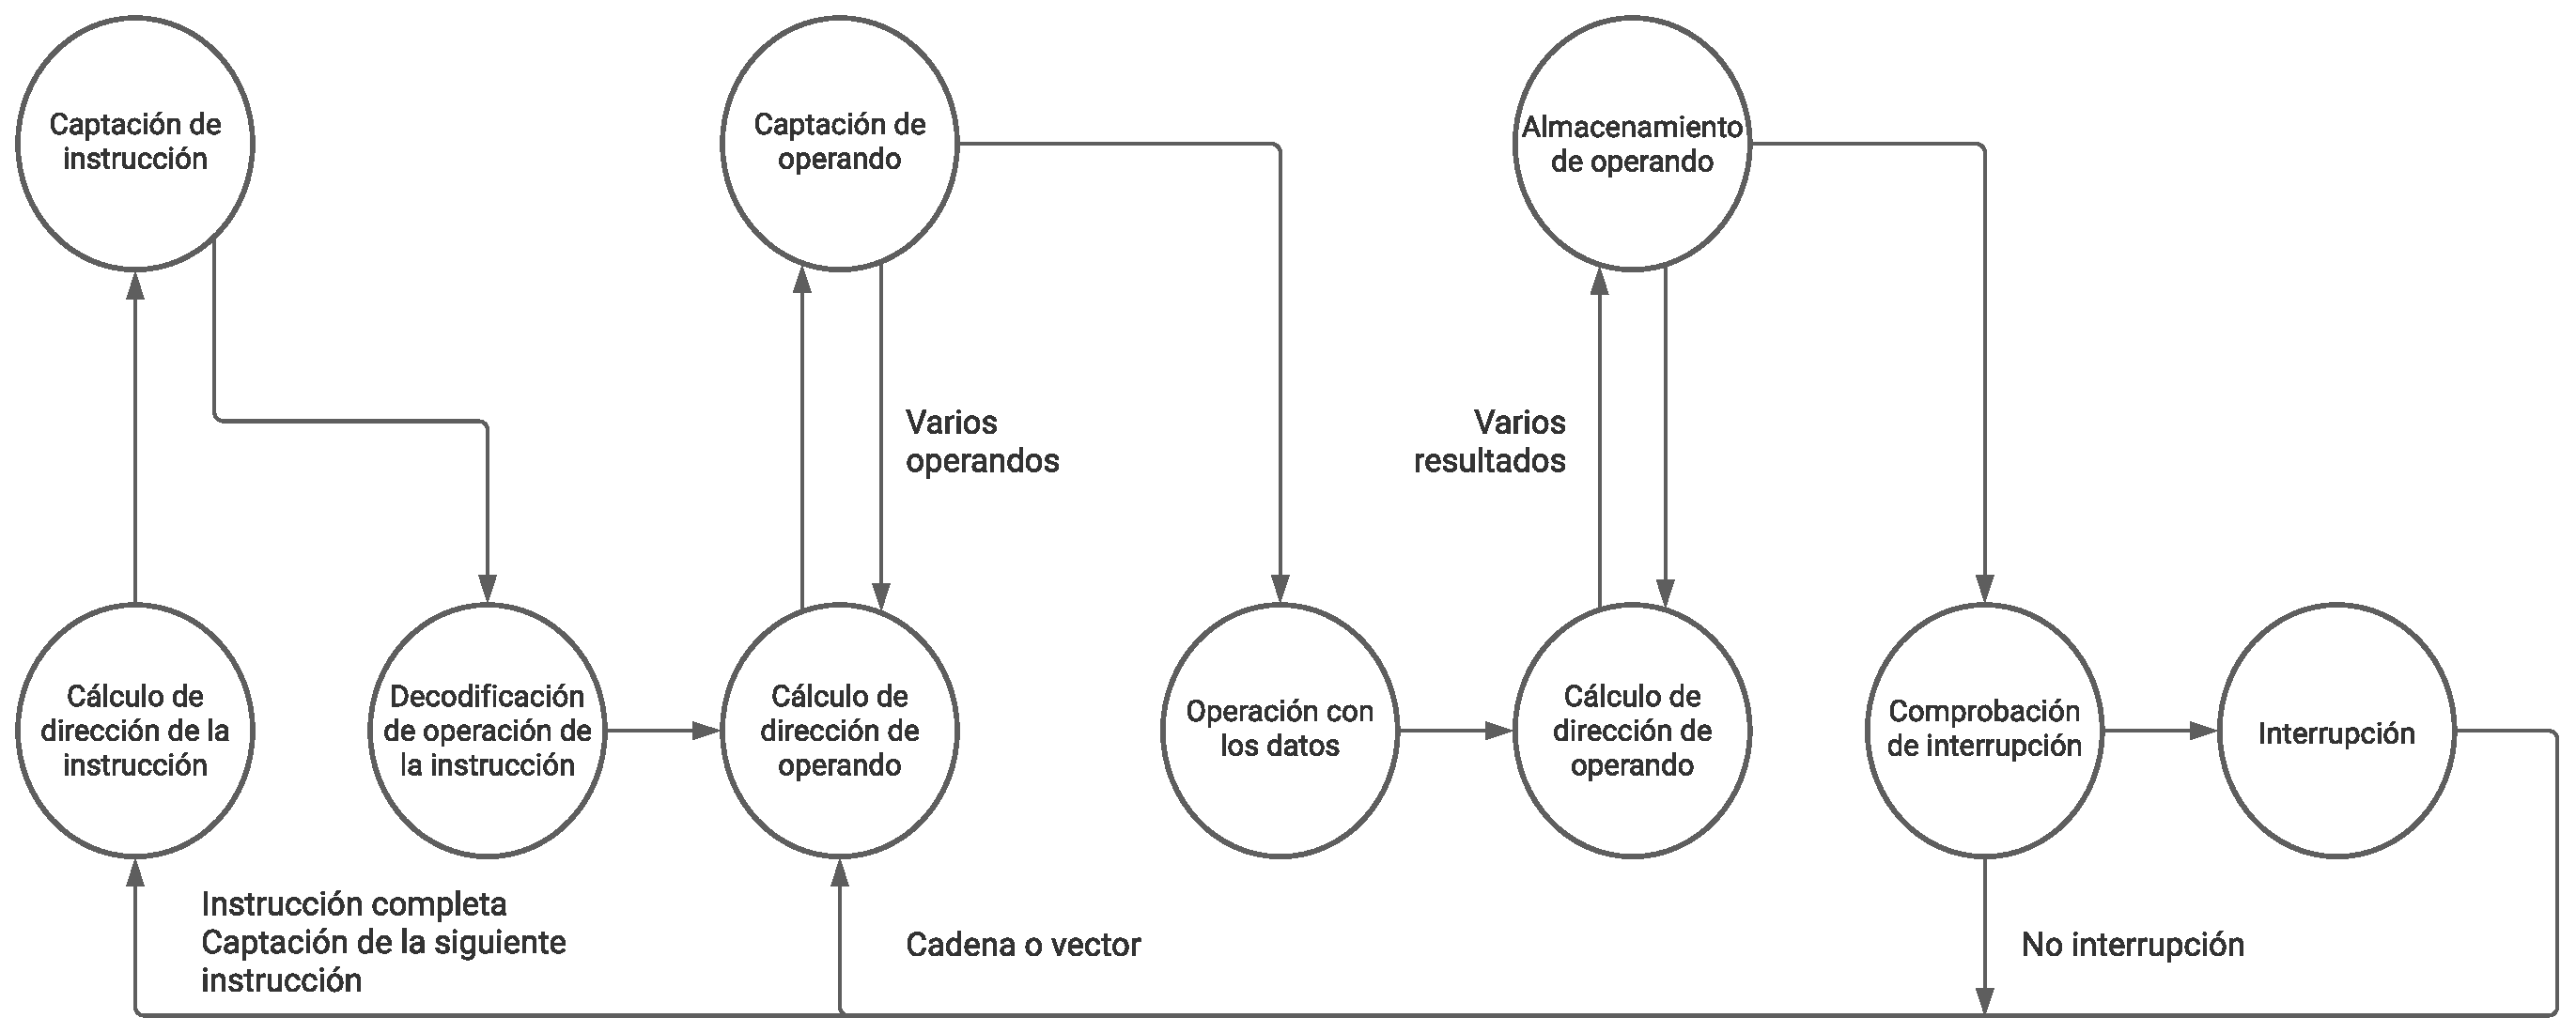
\includegraphics[width=0.8\textwidth]{Ciclo-de-instruccion-STI}
  \caption{Ciclo de instrucción (con interrupciones)}
\end{figure}

\subsection{Tipos de interrupciones}

Podemos clasificar las interrupciones dependiendo de su importancia:

\begin{itemize}
  \item \textbf{No enmascarables}: son aquellas interrupciones que no pueden ser ignoradas. Indican eventos peligros o de alta prioridad y requieren un respuesta eficiente y rápida.
  \item \textbf{Enmascarables}: son aquellas interrupciones que pueden ser ignoradas. Sus eventos no configuran peligro ó pueden esperar. La posible solicitud de interrución puede inhibirse con instrucciones especiales.
\end{itemize}

\begin{subs}
  \subsubsection{Interrupciones por hardware}
  
  Las interrupciones por hardware son las generadas por los dispositivos de E/S. El sistema de cómputo tiene que manejar estos eventos externos `no planeados`. Además, las mismas no están relacionadas con el proceso que se encuentra ejecutándose en ese momento. Son conocidas como \textit{interrupt request}.

  Las \textbf{traps/excepciones} son interrupciones por hardware creadas por el procesador moderno en respuesta a ciertos eventos internos:

  \begin{itemize}
    \item \textbf{Condiciones excepcionales}: overflow en el ALU de punto flotante.
    \item \textbf{Falla de programa}: tratar de ejecutar una instrucción no definida.
    \item \textbf{Falla de hardware}: error de paridad de memoria.
    \item \textbf{Accesos no alineados ó a zonas de memoria protegidas}: acceso a memoria no permitido.
  \end{itemize}

  \subsection{Interrupciones por software}

  Las interrupciones por software son instrucciones explícitas que afectan al procesador de la misma manera que las interrupciones por hardware. La instrucción INT $n$ permite a las interrupciones ser generadas desde dentro del software utilizando el número del vector de interrupción como un operando.

  Estas interrupciones permiten depurar los gestores de interrupción. También se utilizan para invocar funciones del sistema operativo, permitiendo asi cargar subrutinas del sistema operativo en algún lugar y puedan utilizarse.
\end{subs}

\subsection{Interrupciones múltiples}

Hasta ahora únicamente se ha discutido la existencia de una sola interrupción. Sin embargo, es posible que se produzcan varias interrupciones simultáneamente. 
Se pueden seguir dos alternativas para tratar las interrupciones múltiples:

\begin{itemize}
  \item \textbf{Interrupción inhabilitada}: mientras se está atendiendo una interrupción, se deshabilitan las interrupciones. Si se produce una interrupción, queda pendiente y será examinada por el procesador una vez que este haya activado las interrupciones nuevamente.
  El inconveniente de este enfoque es que no teiene en cuenta la prioridad relativa ni las solicitudes con un tiempo crítico. 
  \item \textbf{Interrupciones con prioridades}: se defienen prioridades para las interrupciones y permite que una interrupción de prioridad más alta pueda interrumpir a un gestor de interrupción de prioridad menor. Cuando se ha gestinoado la interrupción de prioridad más alta, el procesador vuelve a las interrupciones previas.
\end{itemize}

\begin{figure}[H]
  \centering
  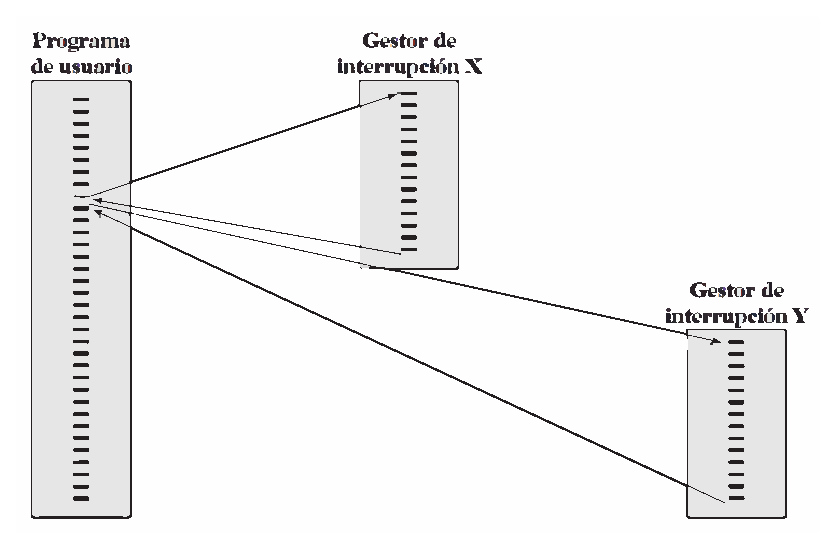
\includegraphics[width=0.8\textwidth]{Interrupciones-secuenciales}
  \caption{Interrupciones secuenciales}
\end{figure}

\begin{figure}[H]
  \centering
  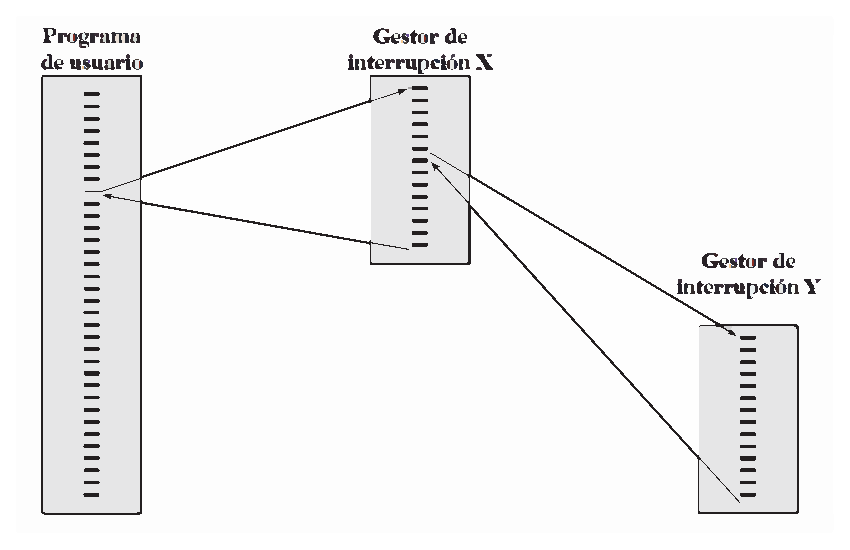
\includegraphics[width=0.8\textwidth]{Interrupciones-anidadas}
  \caption{Interrupciones con prioridades}
\end{figure}

\subsection{Funcionamiento de las E/S}

Un módulo de E/S puede intercambiar datos directamente con el procesador. Igual que el procesador puede iniciar una lectura o escritura en memoria, también puede leer o escribir datos de un módulo de E/S.
En algunos casos, es deseable permitir que los intervambios de E/S se produzcan directamente con la memoria. En ese caso, el procesador cede a un módulo de E/S la autoriadad para leer de o escribir en memoria, para que así la transferencia de E/S-memoria pueda producirse sin la intervención  sel procesador.
Durante esas transferencias, el módulo de E/S proporciona a la memoria las órdenes de lectura o escritura, liberando al procesador de cualquier responsabilidad en el intercambio. Esta operación se conoce con el nombre de \textit{DMA} (Direct Memory Access).